\documentclass[border=10pt]{standalone}

\usepackage{tikz}
\usepackage{tikzsymbols}
\usetikzlibrary{calc,patterns,shapes.geometric}

\def\centerarc[#1](#2)(#3:#4:#5){\draw[#1] ($(#2)+({#5*cos(#3)},{#5*sin(#3)})$) arc (#3:#4:#5);}

\begin{document}
	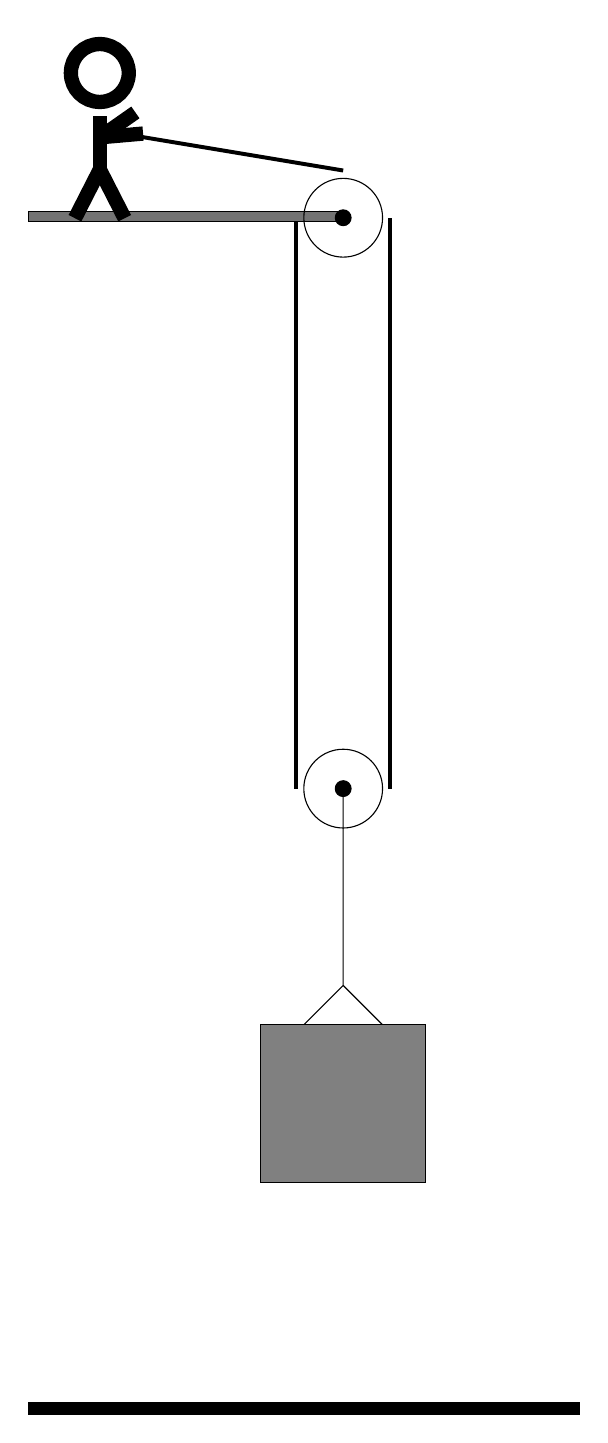
\begin{tikzpicture}
		%%%%% START %%%%%
		\draw[fill=black!55] (-2, 12) rectangle (2, 12.125);
		
		\draw (2, 4.8) circle (0.5);
		\draw[fill=black] (2, 4.8) circle (0.1);
		
		\draw (2, 12.05) circle (0.5);
		\draw[fill=black] (2, 12.05) circle (0.1);
		
		\draw (2, 4.8) -- (2, 2.3) -- (1.5, 1.8) -- (2.5, 1.8) -- (2, 2.3);
		\draw[fill=black!50] (0.95, 1.8) rectangle (3.05, -0.2);
		
		\draw[line width=0.5mm] (1.4, 12) -- (1.4, 4.8);
		\centerarc[line width=0.5mm](2, 4.8)(180:360:0.6);
		\draw[line width=0.5mm](2.6, 4.8) -- (2.6, 12.05);
		\centerarc[line width=0.5mm](2, 12.05)(0:90:0.6);
		\draw[line width=0.5mm](2, 12.65) -- (-1, 13.15);
		
		\node at (-1, 13.15) {\Strichmaxerl[10][-175][35]};
		
		\draw[fill=black] (-2, -3) rectangle (5, -3.15);
		%%%%% END %%%%%
	\end{tikzpicture}
\end{document}